\section{Introduction}\label{sec:intro}

Physics-informed neural networks (PINNs) approximate the solution of a partial
differential equation (PDE) by minimising residuals of the governing equation,
initial and boundary conditions, and available observations at sampled training
points \citep{raissi2019pinns}. Competing loss terms and differential-operator
conditioning can impede optimisation
\citep{wang2021understanding,rathore2024challenges}; collocation strategies can
also fail to propagate initial and boundary information into the interior
\citep{daw2023r3}. Converting a small sampled residual loss into a solution-error
bound requires suitable stability and sampling conditions
\citep{mishra2023generalization}. The remaining
error can be highly non-uniform: a network may approximate the smooth bulk
accurately while retaining substantial error near a thin layer or moving
interface. Domain-averaged diagnostics can conceal this concentration.

Uncertainty estimates could help identify these locally unreliable predictions,
but their interpretation depends on what they describe. In scientific machine
learning, uncertainty may arise from noisy observations, limited information about
model parameters, or numerical approximation error in the computed solution
\citep{psaros2023uq}. These sources need not concentrate in the same parts of
the domain. In particular, uncertainty under a residual-based training model
need not track numerical approximation error.
Bayesian PINNs combine physical constraints with a probabilistic model of noisy
observations and propagate the resulting parameter uncertainty to the solution
\citep{yang2021bpinns}. Deep ensembles use variation between independently trained
predictors \citep{lakshminarayanan2017ensembles}. Whether this predictive spread
tracks numerical approximation error must be assessed rather than assumed.

Local Gaussian methods construct uncertainty around a single trained network
\citep{daxberger2021laplace}. A Laplace approximation uses the Hessian of the
negative log-posterior at a posterior mode. For a Gaussian residual likelihood,
the Gauss--Newton approximation replaces the negative log-likelihood Hessian by
the noise-scaled residual Jacobian Gram matrix, omitting residual second-derivative
terms. With a Gaussian
prior, the resulting covariance is also the exact posterior covariance of the
linearised (affine) residual model at the chosen checkpoint. Linearising the output
propagates this parameter covariance to predictive variances
\citep{immer2021linearized}. In the related setting of neural operators, LUNO
uses model linearisation to propagate Gaussian weight uncertainty into a
function-valued Gaussian process \citep{magnani2025linearization}. This
operator-learning setting differs from our fixed-solution residual model.
\citet{kristiadi2021learnable} show that uncertainty geometry can change while
point predictions remain fixed, motivating a separate assessment of covariance
allocation.

The prior precision and residual-noise variance determine the relative strength
of prior regularisation and residual constraints. Marginal likelihood, or
evidence, integrates the likelihood over the prior and provides a training-based
criterion for selecting these scales \citep{immer2021evidence}.
\citet{antoran2022evidence} account for the difference between a trained
checkpoint and the affine posterior optimum using a fixed network linearisation.
PINN applications already include eikonal travel-time inversion for hypocentre
localisation with diagonal-Fisher curvature \citep{izzatullah2022hypopinn}, and
the heat, wave and Burgers equations with full-Hessian Laplace inference and
evidence-based selection of prior strength and residual weights
\citep{graczyk2026bayesian}. Our regional audit freezes the checkpoint and
relative residual weights, leaving that joint training and hyperparameter-selection
procedure outside the comparison.

Complementary approaches connect uncertainty more directly to numerical accuracy.
Error-Aware B-PINNs incorporate numerical discrepancy into predictive uncertainty
\citep{graf2022erroraware}; solution-error bounds can set spatially varying
likelihood widths in a second Bayesian fitting stage \citep{flores2025errorbounds}.
Calibration assesses whether interval coverage agrees with its nominal level.
Physics-informed conformal prediction uses PDE residuals as nonconformity scores
to calibrate coverage in residual space
without labelled solutions \citep{gopakumar2025calibrated}. Conformal calibration
of PINN predictions uses labelled solution values, with local quantiles allowing
spatially adaptive bands \citep{yu2026conformal}. Marginal coverage guarantees,
under their stated assumptions, do not by themselves ensure coverage conditional
on membership in a sharp region. Section~\ref{sec:discussion} illustrates this
distinction with a split-conformal example. Our contribution is a controlled
regional audit of a full-network residual Gaussian: scale and centre comparisons,
reference feature refits and spectral analysis separate covariance allocation
from interval coverage. Our audit asks how useful this covariance is for describing
deterministic solution error under the specified likelihood.

We study two nonlinear parabolic problems: viscous Burgers, where nonlinear
transport competes with diffusion and produces a thin layer, and Allen--Cahn,
a reaction--diffusion equation with moving phase interfaces. The two architectures
are an independent-feature multilayer perceptron (MLP) and its random-Fourier-feature
variant. For each fixed trained network, we use the Gaussian posterior of the
frozen affine residual and output model. Write $z=(x,t)$ for a space--time point,
$u_\theta(z)$ for the trained prediction and $g(z)=\nabla_\theta u_\theta(z)$ for
its parameter sensitivity. Let $J$ be the Jacobian of the weighted training
residuals and $F=J^\top J$.

\begin{samepage}
For isotropic prior precision $\alpha>0$ and common
weighted-residual variance $v>0$, the parameter covariance $\Sigma$ and latent
predictive variance $\sigma^2$ are
\begin{equation*}
 \Sigma=v(F+\gamma I)^{-1},\qquad
 \sigma^2(z)=g(z)^\top\Sigma g(z),\qquad \gamma=\alpha v.
\end{equation*}
\end{samepage}
The prior variance is $1/\alpha$ in each parameter direction, and $\sigma(z)$ is
the predictive standard deviation, without an added output-noise term. The common
variance is applied after the fixed block weights. At fixed effective
precision $\gamma$, the affine predictive centres and uncertainty contrasts are
unchanged, while widths scale as $\sqrt v$. Our plug-in baseline uses $v=1$ and
$\alpha_0=1/\langle\theta^2\rangle$, with the mean square taken over all trainable
weights and biases; this rule is not evidence maximisation. All these parameters
enter the covariance. The Fourier frequencies are fixed embedding constants and
are excluded from $\theta$ (Section~\ref{sec:setting}).

Reference-gradient percentiles define the sharp and bulk regions, separated by
a transition region (Definition~\ref{def:regions}). We compare sharp-to-bulk
root-mean-square (RMS) uncertainty and error contrasts. Equal contrasts mean equal
relative concentration, without determining absolute width or within-region
coverage. The predictive centre is the prediction around which intervals are
drawn. Because the prior is absent during training, the affine posterior mean
can differ from the trained output. Comparing priors centred at zero and at
$\theta$ isolates shrinkage towards zero from the likelihood correction. We also
evaluate the shifted nonlinear network as a forward diagnostic with covariance
frozen at $\theta$. Reference solutions determine the regions and run admission,
provide evaluation errors, and enter the explicitly reference-informed oracle and feature-refit
diagnostics. At a specified checkpoint and scales, the covariance is formed from
training residuals and network sensitivities.

All $17$ admitted runs have a baseline allocation deficit: uncertainty is less
concentrated in the sharp region than the error (Table~\ref{tab:ceiling};
Figure~\ref{fig:burgers-slice}). This relative deficit coexists with substantial
regional overcoverage. The training-based scale choices change both properties:
with trained centres, the conditional noise maximum-likelihood estimate
under-covers both regions in all eight Burgers--MLP seeds, while finite-grid
evidence selections frequently
reach the lower noise boundary and can be numerically sensitive. Five
Burgers--MLP seeds have identified contrast-matching precisions spanning more
than four orders of magnitude; three retain the deficit throughout the sampled
range.

Centring the prior at the checkpoint retains the baseline deficit in all $17$
runs. Relative to the trained prediction, its affine mean improves full-grid
accuracy in $15/17$ runs at the conditional noise-MLE scales, without calibrating both
regions; nonlinear evaluation instead worsens bulk error in all $17$.
Even an oracle that matches trained-centre
RMS contrasts and calibrates bulk coverage to $68\%$ gives only
$30.3$--$55.7\%$ sharp coverage at the five identified Burgers--MLP matching
points. Thus regional allocation and interval coverage are separate properties.
Readout refits assess feature expressivity, while spectral analysis explains the
scale dependence of covariance allocation.

\begin{figure}[t]
\centering
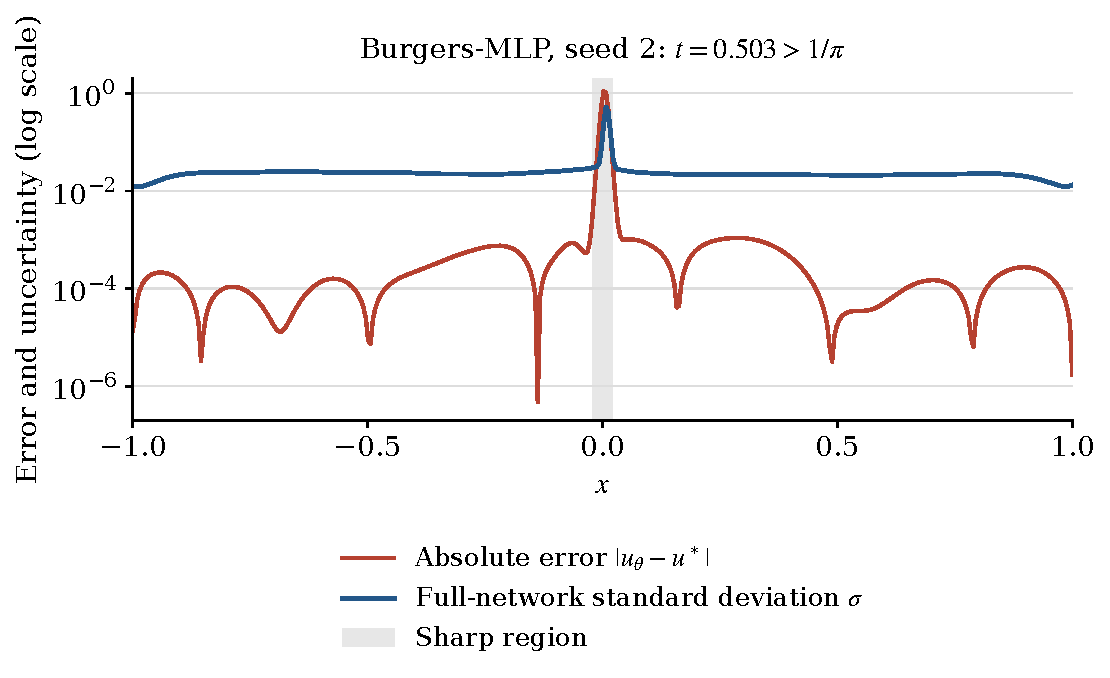
\includegraphics[width=.94\textwidth]{figures/burgers_error_uncertainty_slice.pdf}
\caption{Burgers--MLP seed $2$: absolute error and full-network baseline standard
deviation at $t=0.503$, the stored slice nearest $t=0.5$, after breaking time $1/\pi$.
The logarithmic scale is shared without rescaling; shading marks the global sharp
region of Definition~\ref{def:regions}. Error is more concentrated near the layer.
Here $|e|>\sigma$ near its centre; this is seed-specific, with post-formation calibration
varying across seeds (Table~\ref{tab:temporal}). Full-grid contrasts are in
Table~\ref{tab:ceiling}.}
\label{fig:burgers-slice}
\end{figure}

\begin{samepage}
\emph{Contributions.}
\begin{itemize}
\item \emph{Scale sensitivity and regional coverage (Section~\ref{sec:ceiling}).}
The tested scales and centres do not reliably calibrate both regions. The baseline
deficit survives the alternative prior centre, and direct evaluation at refined
contrast-matching precisions confirms that RMS agreement is insufficient after
bulk calibration.
\item \emph{Reference feature expressivity (Section~\ref{sec:offmanifold}).}
Using reference values to refit the final linear layer leaves below $4\%$ of the trained
sharp-region error energy on held-out time blocks in $16/17$ runs. This tests feature
expressivity independently of residual-only coefficient selection.
\item \emph{Spectral weighting (Section~\ref{sec:theory}).}
A ratio of weighted spectral sums explains scale dependence. In the canonical runs,
covariance weighting amplifies modest regional differences in total tangent norms.
Two-subspace bounds constrain contrast but are too wide to certify the measured
baseline deficit. Lean~4 verifies the spectral bounds and conditional scale limits,
prior-centre bounds and coverage envelopes; reported run counts remain numerical.
\end{itemize}
\end{samepage}

\emph{Empirical scope.}
All eight attempted Burgers--MLP seeds are admitted. Burgers--Fourier,
Allen--Cahn--MLP and Allen--Cahn--Fourier each have three admitted runs selected
by the error criterion in Section~\ref{sec:setting} and are exploratory.
Attempted counts and rejected settings remain explicit. The results concern the
specified training-weighted residual metric and reference-based partition.
